\documentclass{article}

% Language setting
% Replace `english' with e.g. `spanish' to change the document language
\usepackage[english]{babel}

% Set page size and margins
% Replace `letterpaper' with`a4paper' for UK/EU standard size
\usepackage[letterpaper,top=2cm,bottom=2cm,left=3cm,right=3cm,marginparwidth=1.75cm]{geometry}

% Useful packages
\usepackage{amsmath}
\usepackage{graphicx}
\usepackage{pythontex} 
\usepackage{subfig}

\usepackage[colorlinks=true, allcolors=blue]{hyperref}
\usepackage{qcircuit}
\usepackage[ruled,vlined]{algorithm2e}
\usepackage[utf8]{inputenc}
\usepackage{tcolorbox}
\newtcbox{\inlinecode}{on line, boxrule=0pt, boxsep=0pt, top=2pt, left=2pt, bottom=2pt, right=2pt, colback=gray!15, colframe=white, fontupper={\ttfamily \footnotesize}}


\title{IonQ Application Team Homework}
\author{Shangjie Guo}

\begin{document}
\maketitle

\section{Strategy}

\subsection{Airbus QC challenge 2019}
\textbf{Airbus set up a quantum computing challenge in 2019 with five problems (\url{https://www.airbus.com/content/dam/corporate-topics/innovation/Airbus-Quantum-Comp uting-Challenge-Problem-Statements.pdf}). Pick one of the problems and give a high-level overview of how you would approach it with a quantum computer. Think about parameters such as computational efficiency, ease of adoption, and years to feasibility.}\\

\noindent \textit{Problem choosing:} These 5 problems can be classified into 2 classes: Optimization of continuous variables (Problem 1, 4, 5) and Efficient differential equation solver (Problem 2, 3). I believe both classes are hard for NISQ devices. But I think PDE solver should be more realistic, because intuitively I think digital quantum computers are great for solving PDEs (at least for some particular ones) since Schrodinger equations are PDEs after all. I choose \textbf{Problem 2: Computational Fluid Dynamics} since I found a relevant paper that looks promising and potentially improvable.\\

\noindent \textit{Problem solving:} To solve the problem I will search for related existing papers, this one is the most relavent: \url{https://www.nature.com/articles/s41534-020-00291-0}. It claims that with quantum amplitude estimation,  Navier–Stokes equations (NSE) discretized with finite volume method (FVM) can be solved more efficiently, solving discretized NSE  are commonly used on simulating CFD. According to this paper, this method can solve both viscous and inviscid flows. The result presented in the paper is about 1-D flow, while the author claims ``a similar discretization procedure can be used to reduce an arbitrary set of PDEs to a corresponding
set of ODEs.''\\

\textbf{Method implementation: 
}
The core algorithm of this method is quantum Fourier transformation (QFT) so I will estimate resource cost based on QFT. QFT implementation requires full qubit connectivity, thus we may want to use ion trap devices. 

Computational efficiency:
The paper claims that quantum speed-up is more significant for rough /nonsmooth CFD cases. In the rough limit, this quantum algorithm  has a \textit{squareroot} reduction in $\epsilon$-complexity over the classical random algorithm. 


Ease of adoption: For a 11-qubit device with full connectivity (IonQ device on AWS Braket). We can use this paper for 5 volume elements (5 for QFT and 5 for contorl ancillae and measurement). The circuit depth for approximated QFT is 8 (approximation degree $=2$, for method in \url{https://arxiv.org/abs/quant-ph/9601018}). Assume embedding and controlled rotation only consist circular two local CNOTs, each should have depth $<10$. With inverse QFT, the total circuit depth should be $<35$ and can be further reduced by transpiler and other techniques. 1024 shots per run should be sufficient for 5 qubit state tomography (may also be reduced), according to AWS braket, that should be about \$10 per experiment. That concludes this algorithm should not be hard to implement for small quantum device.


Years to feasibility: For useful CFD simulation we may need at least $10^2\sim 10^3$ descritized volume, also twice as large sized quantum computer, which is possible in 5 years according to IBM \& IonQ roadmap. Since circuit depth for Approximate QFT scales up logarithmly with number of qubits used, significant boost in gate fidelity can benefit but only necessary for implementing this method.

\textbf{Some thoughts for improvement:}
\begin{enumerate}
    \item Intuitively, NSE descritized with FVM seems only contain nearest neighbor interaction, maybe a full QFT (also full connectivity) is not necessary.
    \item Solving the eigen-function with lowest eigen-energy of NSE with VQE-ish algorithm may also be useful for some dissipative cases.
    \item It might be possible to divide-and-conquer a larger fluid system discretized with FVM into smaller subsystems and preserve important dynamics. For example, this paper shows this idea could be possible (It used small neural network repetitively to control and predict a large classical chaotic system): \url{https://journals.aps.org/prl/abstract/10.1103/PhysRevLett.120.024102}.
\end{enumerate}


% Test: Simulator test Small scale QC test




\newpage
\subsection{First demonstration of quantum advantage}
\textbf{According to you, in which application area will we see the first demonstration of quantum advantage and why? Try to take into account the latest advances in algorithm and hardware development when presenting your answer.}\\

According to Google and USTC, we have achieved quantum advantage for random number generation and Boson sampling. And in my opinion, the first ``useful'' demonstration of quantum advantage might be using quantum simulation (or VQE) to find ground state configurations of a set of complex molecules, if we define ``useful'' as ``profitable''. 

Here are my reasoning: 

\begin{enumerate}

\item Deep circuits are bad, therefore algorithms related to time evolution and Trotterization (QAOA) might be harder, and solve time invariant  eigenvalues/eigenstates might be easier.

\item We may design certain QC hardware topology for certain type of molecule Hamiltonian and ansatz. Changing QC topology without changing device might be possible for cold atom lattices or even ion traps. 

\item Physicists may found specific QC designs faster if the task itself is quantum related. 

\item We may design the ansatz to make the circuit shallower if we only interested in a certain sub-Hilbert space, or global ground state is not important.

\item Interactions within a molecule are local, we may not need long range interactions to find its ground state.

\item Bonus: Also it is related to what Richard Feynman first suggested: ``if you want to make a simulation of nature, you’d better make it quantum mechanical''.
\end{enumerate}


\newpage
\section{Technical}
\subsection{1D Heisenberg model with CNOT}

\textbf{Consider the Heisenberg model on a 1D lattice with nearest neighbor interactions. Construct a circuit that allows you to do a Trotterized time-evolution of this Hamiltonian using single qubit rotations and CNOT gates. Make it as efficient in the number of 2-qubit gates and circuit depth as you can. Then use a quantum software framework of your choice (for example, Qiskit or Cirq) to implement this and show the code.}\\

Consider a general Heisenberg model (XYZ model):

\begin{equation}
    H = \sum_j J_x \sigma_x^j \sigma_x^{j+1} + J_y \sigma_y^j \sigma_y^{j+1} + J_z \sigma_z^j \sigma_z^{j+1} + \frac{h}{2} \sigma_z^j
    \label{eqn:hal1}
\end{equation}

Then the Trotterized time-evolution operator for time $T$ of Hamiltonian \ref{eqn:hal1} is:

\begin{align}
    U = &[e^{-i(ht/2) \sum_j \sigma_z^j}e^{-it \sum_j J_x \sigma_x^{2j} \sigma_x^{2j+1} + J_y \sigma_y^{2j}+ \sigma_y^{2j+1} + J_z \sigma_z^{2j}\sigma_z^{2j+1}}\\
    &\times e^{-it \sum_j J_x \sigma_x^{2j+1} \sigma_x^{2j+2} + J_y \sigma_y^{2j+1}+ \sigma_y^{2j+2} + J_z \sigma_z^{2j+1}\sigma_z^{2j+2}}]^n
    \label{eqn:hal1}
\end{align}

where $t=T/n$ is the Trotterized time step. There can be extra Trotterization error introduced since the second and last term are not commute. For one time step, a 4 qubit circuit looks like:

\[
\begin{array}{c}
\Qcircuit @C=1em @R=.7em {
& \gate{R_z(ht)} & \multigate{1}{N(\vec{J}t)} & \qw & \qw \\
& \gate{R_z(ht)} & \ghost{N(\vec{J}t)} & \multigate{1}{N(\vec{J}t)} & \qw \\
& \gate{R_z(ht)} & \multigate{1}{N(\vec{J}t)} & \ghost{N(\vec{J}t)} & \qw \\
& \gate{R_z(ht)} & \ghost{N(\vec{J}t)} & \qw & \qw 
}
\end{array}
\]

According to \url{https://arxiv.org/abs/quant-ph/0308006}, Operator $N(\vec{J}t) = \exp(-it J_x \sigma_x^0 \sigma_x^1 + J_y \sigma_y^0 \sigma_y^1 + J_z \sigma_z^0 \sigma_z^1)$ can be decomposed to CNOT and single rotation gates as the following circuit:

\[
\begin{array}{c}
\Qcircuit @C=1em @R=.7em {
& \qw & \targ & \gate{R_z(\gamma)} & \ctrl{1} & \qw & \targ & \gate{R_z(-\pi/2)} & \qw\\
& \gate{R_z(\pi/2)} & \ctrl{-1} & \gate{R_y(\alpha)} & \targ & \gate{R_y(\beta)} & \ctrl{-1}& \qw & \qw
}
\end{array}
\]

Where $\alpha = 2J_x t+\pi/2$, $\beta = -2J_y t-\pi/2$, $\gamma = -2J_z t-\pi/2$. Next, each time step of 1-D XYZ model can be decomposed to circuit with depth = 11 (6 if $n=2$) and number of CNOT gate = $3(n-1)$, where $n$ is the number of sites. A 4 qubits example as illustrated below:

\[
\begin{array}{c}
\Qcircuit @C=1em @R=.7em {
& \gate{R_z(ht-\pi/2)} & \targ & \gate{R_z(\gamma)} & \ctrl{1} & \qw & \targ & \qw & \qw & \qw & \qw & \qw & \qw \\
& \gate{R_z(ht)} & \ctrl{-1} & \gate{R_y(\alpha)} & \targ & \gate{R_y(\beta)} & \ctrl{-1} & \targ & \gate{R_z(\gamma)} & \ctrl{1} & \qw & \targ & \qw \\
& \gate{R_z(ht)} & \targ & \gate{R_z(\gamma)} & \ctrl{1} & \qw & \targ & \ctrl{-1} & \gate{R_y(\alpha)} & \targ & \gate{R_y(\beta)} & \ctrl{-1} & \qw \\
& \gate{R_z(ht+\pi/2)} & \ctrl{-1} & \gate{R_y(\alpha)} & \targ & \gate{R_y(\beta)} & \ctrl{-1} & \qw & \qw & \qw & \qw & \qw & \qw
}
\end{array}
\]

First $R_z$ of the first qubit included the last $R_z(-\pi/2)$ rotation in $N(\vec{J}t)$ operation from the previous step. This result can be generalized to the case that $h$ and $\vec{J}$ are not constant for each site without changing the depth or counts of CNOT.

There also can be further circuit reduction by using qiskit Transpiler API or the method discussed in  \url{https://www.pnas.org/content/115/38/9456.short}.

\newpage
Here is a Qiskit implementation of circuit described above:
\begin{figure}[h]
    \centering
    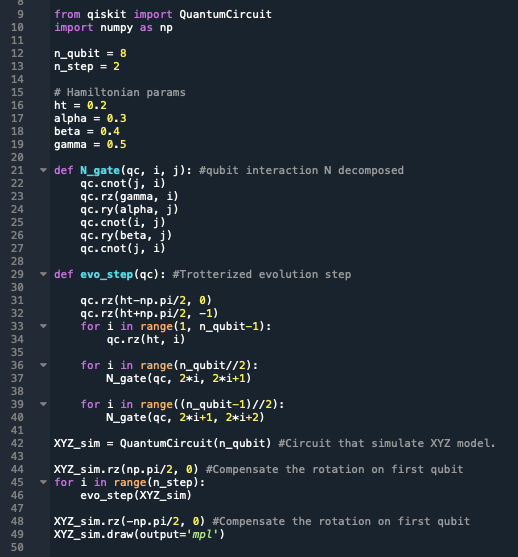
\includegraphics[width=0.7\linewidth]{figt1-2.png}
\end{figure}


Output:
\begin{figure}[h]
    \centering
    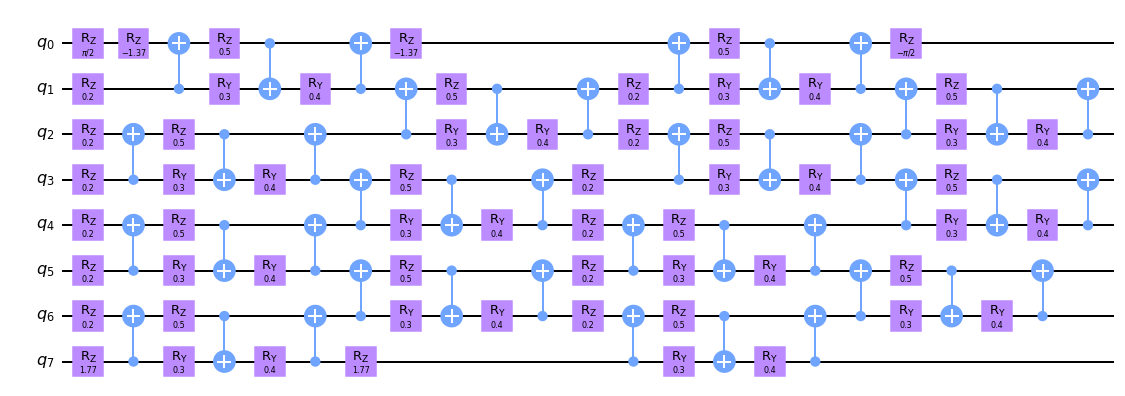
\includegraphics[width=0.8\linewidth]{figt1-3.png}
\end{figure}

\newpage
\subsection{QAOA on square lattice for 3-regular graphs}

\textbf{Consider the QAOA algorithm applied to the MaxCut problem on 3-regular graphs. Suppose you have a square lattice of qubits with nearest neighbor connectivity. Describe an algorithm and write commented pseudocode that allows you to map the qubits in the QAOA circuit to the physical qubit layout and schedule the circuit in the most efficient way you can come up with. Do a theoretical or numerical analysis of the time complexity of the schedule.}\\

According to \url{https://arxiv.org/abs/1703.06199}, for shallowest QAOA, we can at least achieve 0.5293 approximation ratio. That is the best analytical solution I can found. And here I provide a solution that can find a local optimal layout.

I will assume that QAOA will perform better if the \textit{longest} edges of 3-regular graph remapped to the square lattice is shorter. The key idea is starting at a random layout, and for each optimization step: randomly select one of the longest edges and make it shorter by swapping one end with its neighbor, keep doing so until the length of longest edge converges. For example, for $n=50$, this schedule can find a layout with longest edge $L_{\text{max}}=3$ within 2000 steps. (The code to plot this figure is showed on the next page)
\begin{figure}[h]
    \centering
    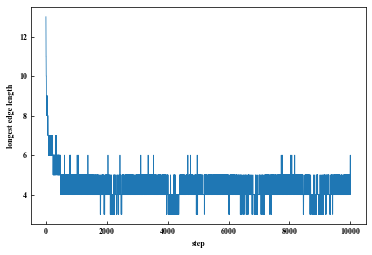
\includegraphics[width=0.5\linewidth]{figt2-1.png}
\end{figure}

With hash-based search, I have reduced the time complexity for each step is linear to number of nodes $n$. And I use numerical method to estimate the step needed to converge ($t_c$). In following plots, I show how $L_{\text{max}}$ and $t_c$ changes with $n$, averaged of 10 graphs for each point plotted. I observed 2 trends: (1) $L_{\text{max}}\propto \sqrt{n}$, which makes sense for square lattice; and (2) $t_c$ looks increasing roughly linearly with $n$, and have local maxima when $L_{\text{max}}$ is increasing to the next integer. Therefore, the total complexity of finding a layout with my schedule is about $O(n^2)$.

\begin{figure}[h]
    \centering
    \subfloat{{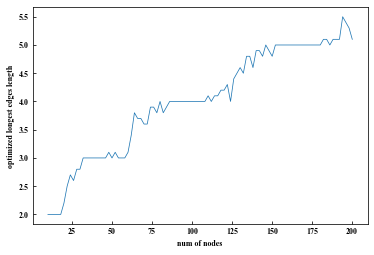
\includegraphics[width=.4\linewidth]{figt2-2.png} }}%
    \qquad
    \subfloat{{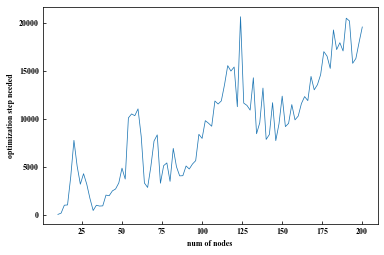
\includegraphics[width=.4\linewidth]{figt2-3.png}}}%
\end{figure}
The good news of my solution are that (1) it can be generalized to any unweighted graphs. (2) I can make a small tweak to sacrifice some accuracy for even shallower circuit (for example: we can ignore the longest $k$ edges, and make the $(k+1)$th longest edge as short as possible, only by changing the \inlinecode{max(list(...))} in line 36 and 74 to \inlinecode{list(...)[np.argmax(list(...))[-k-1]]}).

\newpage
Code for 2.2:
\begin{figure}[h]
    \centering
    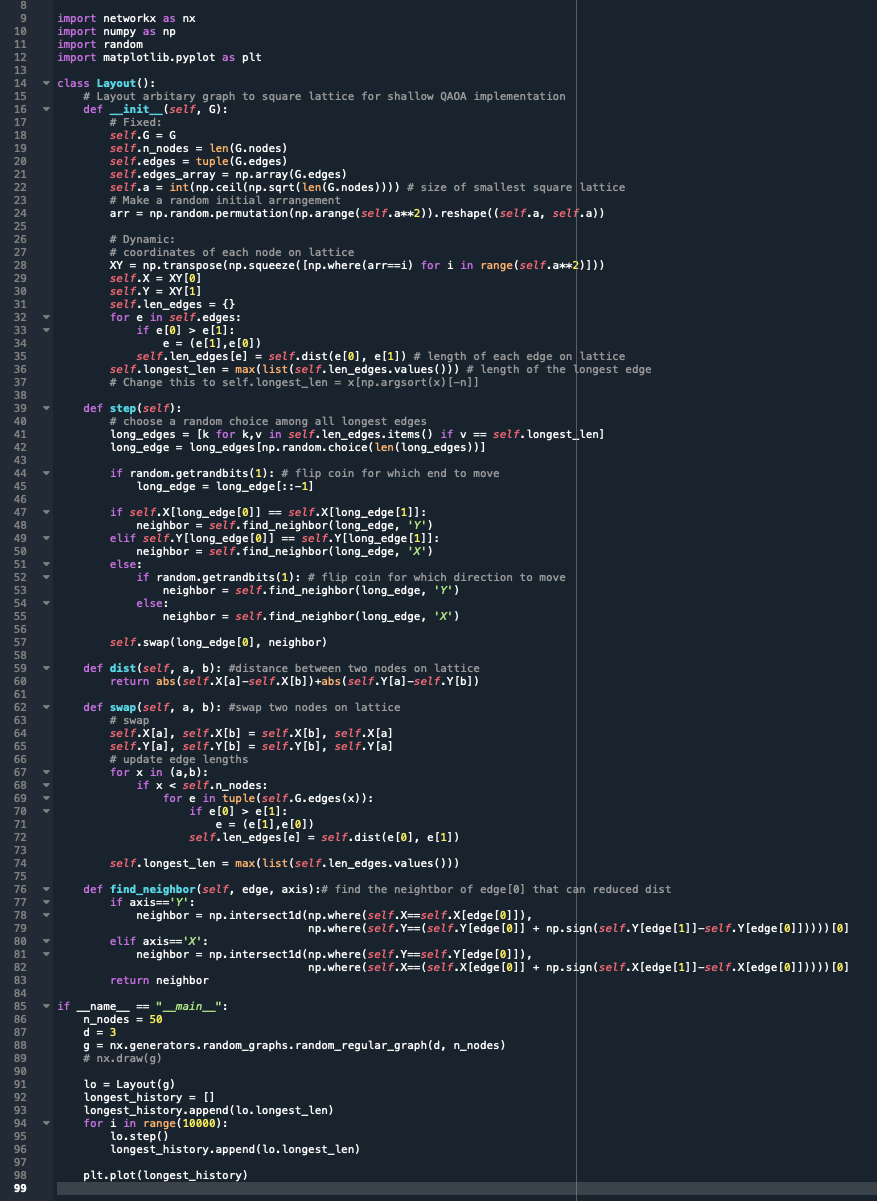
\includegraphics[width=0.87\linewidth]{figt2-4.png}
\end{figure}


\newpage
\subsection{Performance analysis of QAOA}

\textbf{Consider the QAOA algorithm. For uniform graphs, there is numerical evidence (\url{https://arxiv.org/pdf/1812.01041.pdf}) that the approximation ratio will increase exponentially with the number of layers in the algorithm. Assuming this is true, let’s say you have a quantum computer in which depolarizing noise affects each 2-qubit gate. Analyze how the approximation ratio behaves as a function of the strength of the noise and the number of layers.}\\

To use the result is the cited paper, here I will only give an estimation. For more accurate result, we need to do numerical simulations.

From the paper, for an ideal circuit, $r_I \propto 1-\exp (-p/p_0)$, where $r_I$ is approximation ratio, $p$ is the number of layers and $p_0$ is a constant that may related to number of qubits $N$.

To model depolarization noise, I use the equation in Preskill's lecture note:

\begin{equation}
    \rho = (1-q)\rho_I +\frac{q}{3} (\sigma_x\rho_I\sigma_x + \sigma_y\rho_I\sigma_y + \sigma_z\rho_I\sigma_z) 
\end{equation}

Where $q$ is the probability for error occurs within one layer of QAOA. After $p$ layers, the probability of $\rho=\rho_I$ is (perturbation to the 2nd order of $q$, for $p\geq 2$): 

\begin{align}
    \label{error}
     P(\rho=\rho_I) &\approx (1-q)^p + 3C_p^2 (1-q)^{(p-2)}(\frac{q}{3})^2\\
     &\approx 1 - pq +\frac{2p(p-1)}{3}q^2
\end{align}

The first term in \ref{error} represents no error occur in the whole circuit (IIIIII) and second term describe the possibility that an error occurred and corrected by an following error (e.g. IXIIXI). Therefore, the expectation value of QAOA on noisy device is: $F = C \rho = P(\rho=\rho_I)  C \rho_I = P(\rho=\rho_I) F_I$. And since $r = F/C_{\text{max}}$,  $r_I = F_I/C_{\text{max}}$:
\begin{align}
    r = P(\rho=\rho_I) r_I \propto  [1 - pq +\frac{2p(p-1)}{3}q^2](1-e^{-p/p_0})
    \label{res:3}
\end{align}

Again, this is just an estimation with given information, too many assumption are made. And we cannot even directly measure $p_0$, which numerically related to the number of qubits. Simulation is needed for more accurate optimization of $p$, and eqn. \ref{res:3} tell us where to simulate as a start.

Here is the visualization for $r(q, p)$ and $r_\text{opt}(q)$ for $p_0 = 4$ (number of qubits $= 20$ according to the paper), red line indicates optimal depth $p_\text{opt}$. Perturbation approximation breaks at about $pq \geq 1$, which is not included in this plot. As we expected, larger noise leads to shallower $p_\text{opt}$.
\begin{figure}[h]
    \centering
    \subfloat{{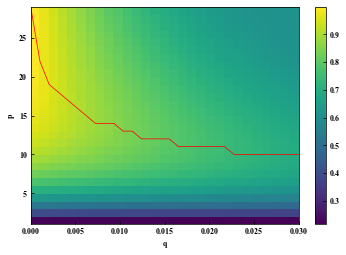
\includegraphics[width=.45\linewidth]{figt3-1.png} }}%
    \qquad
    \subfloat{{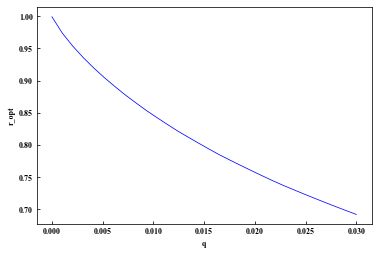
\includegraphics[width=.4\linewidth]{figt3-2.png}}}%
\end{figure}

\end{document}